\documentclass[border=4pt]{standalone}
\usepackage{amsmath,amssymb,amsfonts}
\usepackage{xcolor,colortbl,array,booktabs,multirow}
\usepackage{tikz}
\usetikzlibrary{arrows, automata, backgrounds, calendar, chains, decorations,
    matrix, mindmap, patterns, petri, positioning, shadows, shapes.geometric,
    trees, shapes, decorations.pathreplacing, calc, tikzmark, arrows.meta}
\newcommand{\st}{\text{ s.t. }}
\newcommand{\x}{\mathbf{x}}
\renewcommand{\b}{\mathbf{b}}
\newcommand{\A}{\mathbf{A}}
\newcommand{\R}{\mathbb{R}}
\newcommand{\RR}{\mathbb{R}}
\newcommand{\Z}{\mathbb{Z}}
\newcommand{\ZZ}{\mathbb{Z}}
\begin{document}
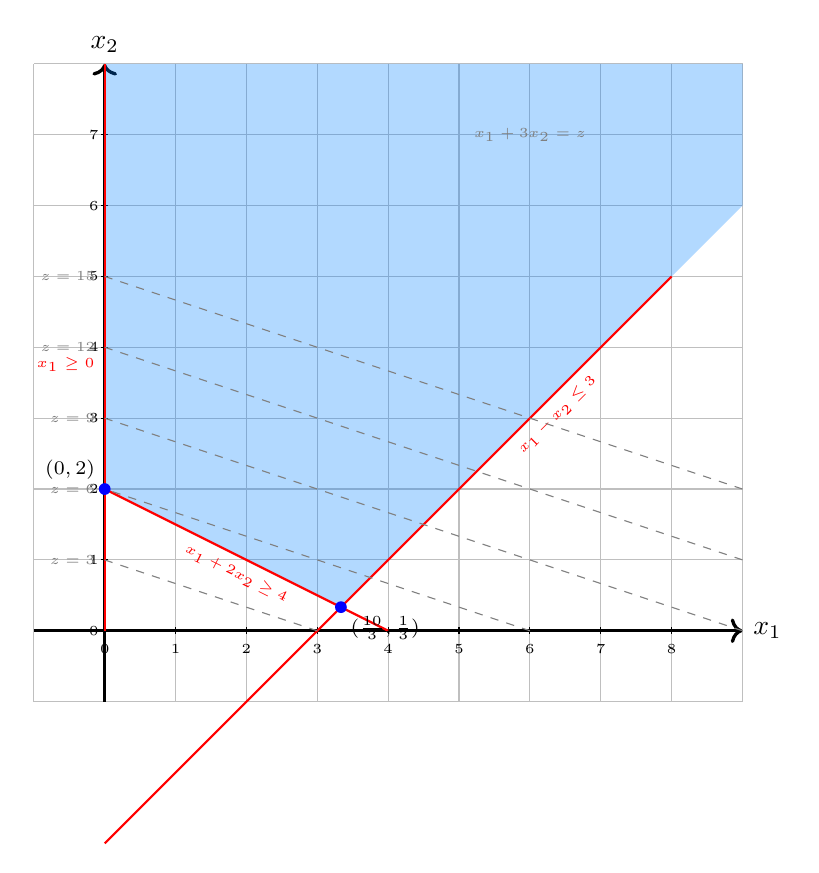
\begin{tikzpicture}[scale = 0.9]
    \draw[gray!50, thin, step=1] (-1,-1) grid (9,8);
    \draw[very thick,->] (-1,0) -- (9,0) node[right] {$x_1$};
    \draw[very thick,->] (0,-1) -- (0,8) node[above] {$x_2$};

    \foreach \x in {0,...,8} \draw (\x,0.05) -- (\x,-0.05) node[below] {\tiny\x};
    \foreach \y in {0,...,7} \draw (-0.05,\y) -- (0.05,\y) node[left] {\tiny\y};

    % Feasible region (unbounded upward-right)
    % Vertices: (0,2), (10/3, 1/3), then extends along both boundary lines
    \fill[blue!50!cyan,opacity=0.3] (0,2) -- (10/3,1/3) -- (9,6) -- (9,8) -- (0,8) -- cycle;

    % Constraint lines
    \draw[red,thick] (0,-3) -- node[below right,sloped,pos=0.7] {\tiny$x_1 - x_2 \leq 3$} (8,5);
    \draw[red,thick] (4,0) -- node[below left,sloped,pos=0.3] {\tiny$x_1 + 2x_2 \geq 4$} (0,2);
    \draw[red,thick] (0,0) -- node[below left] {\tiny$x_1 \geq 0$} (0,8);

    % Level curves (x1 + 3x2 = z)
    \draw[dashed,gray] (3,0) -- (0,1) node[left] {\tiny$z=3$};
    \draw[dashed,gray] (6,0) -- (0,2) node[left] {\tiny$z=6$};
    \draw[dashed,gray] (9,0) -- (0,3) node[left] {\tiny$z=9$};
    \draw[dashed,gray] (9,1) -- (0,4) node[left] {\tiny$z=12$};
    \draw[dashed,gray] (9,2) -- (0,5) node[left] {\tiny$z=15$};

    \node[gray] at (6,7) {\tiny$x_1 + 3x_2 = z$};

    % Vertices
    \node[blue] at (0,2) [circle,fill,inner sep=1.5pt]{};
    \node[blue] at (10/3,1/3) [circle,fill,inner sep=1.5pt]{};
    \node[black,anchor=south east] at (0,2) {\scriptsize$(0,2)$};
    \node[black,anchor=north west] at (10/3,1/3) {\scriptsize$(\tfrac{10}{3},\tfrac{1}{3})$};
\end{tikzpicture}
\end{document}
